\chapter{Evaluation}
The systemC model works as supposed. The output of the algorithm is satisfying and corresponding to the output of the C/C++ application, see figure \ref{fig:result_sysml}. 

\begin{figure}[H]
\centering
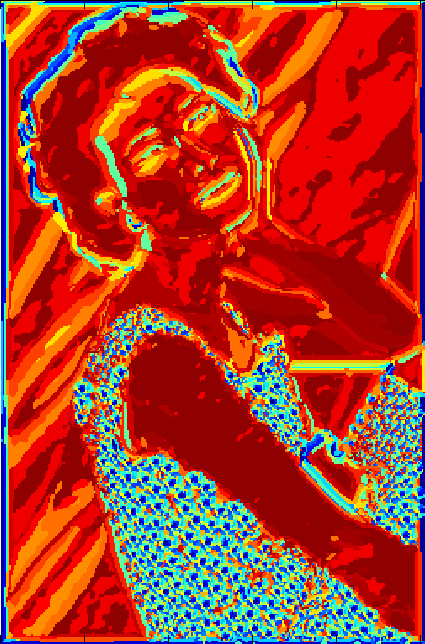
\includegraphics[width = 0.4\linewidth]{result_sysml}
\caption{Resulting image from the systemC model}
\label{fig:result_sysml}
\end{figure}

 
After the BCAM it became clear that the amount of memory is not adequate why an implementation of the k-means classification in hardware will not be enough to increase the computational speed. 
Even though this conclusion is disappointing the advantage in making a model before implementation is very clear. 
The top-down aproach creates a great overview of the problem and makes sure that developers do not focus too much on implementation details and platforms.

To reach the requirements for this project; especially the non-functional requirement that the execution time should be less than 1 minute, another platform has to be considered. 
Hereby it is also beneficial that no developers started implementing the existing C/C++ application directly into a hardware/software system on an already available platform as the DE2 board from Altera.
